\documentclass[10pt,twocolumn]{article} 

% use the oxycomps style file
\usepackage{oxycomps}

% read references.bib for the bibtex data
\bibliography{references}

% include metadata in the generated pdf file
\pdfinfo{
    /Title (Comps Proposal Paper)
    /Author (Sammy Sanchez)
}

% set the title and author information
\title{CS COMPS Proposal Paper}
\author{Sammy Sanchez}
\affiliation{Occidental College}
\email{sanchezs@oxy.edu}

\begin{document}

\maketitle

\section{Problem Context}

For the project that I am doing, I want to make it easier for people that look at sports statistics to visualize the data on graphs to evaluate players. This will be a website or web app that can help people analyze sports players for fantasy sports that helps them pick the best player of their choice for their chosen stats. The user would be able to pick and group stats of the sport they are playing fantasy in and pick a player the want to compare those stats to. A scatter graph will be created to show where the player's data is at and if other players have similar stats. The stats used for the graph will also be in a chart below the graph to see the data. The user would be able to visualize and evaluate the players that are similar to the chosen player and decide on if they would use the player in fantasy sports for their team. The way the user picks that stats will also have a description of how the stat chosen is calculated to give more detail because a person might not know how it is calculated and what is used to calculate it. An example would be True Shooting stat in basketball and would read "TS\% stands for True shooting percentage and it is a measure of shooting efficiency that takes into account field goals, 3-point field goals, and free throws". It will also help users that are interested in sports analytics because of how the app will be a unique way of combining stats to visualize a spectrum of where players line up against each other. It will also be different compared to other databases because of the ability to include stats like body height, weight and age to evaluate players. 

There are no fantasy sports apps that analyzes stats that the users pick specifically and displays it on a graph. Fantasy apps currently only display stats on data charts which makes it hard to virtually analyze stats. Being able to visualize stats and players with specific stats chosen will help any fantasy team owner when picking players for their team. The help will come when a fantasy team owner wants to get a player that is similar to another player statistically and it will help generate points for the team over the season. When the best players are chosen by other teams, it gets harder to find players that produce the same amount of fantasy points and this will help target stats that produce points. Being able to group important stats together will help the owner to see how good other players are to a player that does well in the sport. The graph will show a correlation of the stats picked for evaluation, and it will help drive a decision of what player to pick for the team. 

My project would be useful for fantasy players because it will give them an understanding of how different NBA players can be similar statistically which can help a fantasy team accumulate points over the season. It is helpful when the so called "super stars" are picked in the first couple rounds of a fantasy draft and that there are other players available that have similar statistics to those stars which can help make a positive impact on your team. The impact this project would have on positive players is how they view these NBA players based on what stats they want to compare and teach them about impact players that are not considered stars. 


\section{Technical Background}


For my approach of doing this project, I need to learn how to create a website that can query data from sports stats websites like Sports Reference created by Sean \textcite{sportsReference} and ESPN created by Bill \textcite{espn}. When querying the data it will allow the user to gather those stats from the database websites and create a graph based on the chosen stats. I would have to learn how to create graphs from the gathered data using Python or another coding language that can create graphs. I would need to use an algorithm that can group stats together and make plots on a graph that uses the stats for each player that is being compared. The mathematical equations used would have to be programmed to be implemented when creating the graph based on that stats chosen and might require an algorithm to do it. When the mouse is over the data point, it would have to be programmed to show the player's name on the point. Below the graph would also show the stats used in a chart with other players names. This could be done with querying to select stats from the sports statistic websites and display them on a chart generated from the query. For selecting stats and the player, I would have to program the website to have drop down lists that display all the possible options to choose from.

The way people perceived sports data/statistics over the years has changed drastically because of how reliable sports stats have become for professional teams. In an article written by Alyssa \textcite{sportsStats}, she discusses how sports stats were not used as heavily going back to the 1980's and 90's because of subjective gut feelings about players. These were usually biased because of how a coach or front office person would feel about that player. In 2002, she discussed how the Oakland Athletic in the MLB used statistical analysis to created a baseball team of lesser-known players to have a great season and make the playoffs and many people frowned upon the idea of using statistical analysis to make a team that way. Now, sports statics analysis has taken over how fans and employees of these professional teams views players and evaluate them. Many companies have made their own algorithms to track almost all aspects of a respective sport and evaluate the data that they keep track of. 

Another way people have used sports statistics is to predict MVP awards using algorithms and machine learning. In an article written by David \textcite{MVPpredict}, he discusses the way the NBA MVP is awarded based on the people the vote for it and how an AI can predict who is going to win it. The algorithm compares historical data of past MVP winners through two different equations and sees how accurately the AI predicts the MVP. It used MAE (Mean Absolute Error) and R² (coefficient of determination) to evaluate the the MVP as seen in Figure 1. The experiments that were used was to see if it correctly identified the MVP for a specific year and would calculate the accuracy of guessing the MVP correctly. 

\begin{figure}
    \centering
    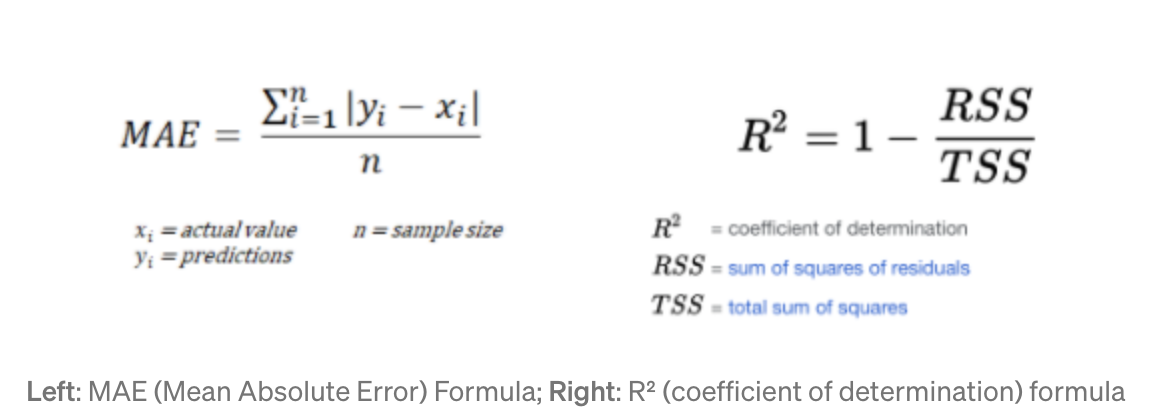
\includegraphics[width=.95\linewidth]{stats.png}
    \caption{
        MAE and R²
    }
    \label{fig:second-page-1}
\end{figure}


\section{Prior Work}

The prior work that has been done is a website called "NBA Player Performance and Scouting Explorer" and the website is created by \textcite{dash}.
It is designed to be used as a way to view and group NBA players with stats on graphs. One of the graphs uses body weight and height as a way to group players with higher physicality or you can group the player strictly off statistics. The players are grouped in the graph based on their position in basketball and a player is selected to be compared to with a chart listed below the graph with the stats. It allows the user to also group players based on the custom stats they choose to evaluate players. Another option to use in this app is how stats picked are grouped together and groups are made for players that are similar with those stats. It is something similar with what I want to do with my project, but in this app, the stats that can be used are limited and I want to expand it with more. It is also only used for basketball players and I would expand it to other sports like baseball and football. In Figure 2, it shows the visualization of Steph Curry compared to other players in the NBA that have a similar physicality to him, but also shows how statistical data compared to him as well. The inspiration for this website can be to find good NBA players and be unbiased using their app. As a user, they can pick their favorite player and compare them to other players using stats or physicality of the chosen player and the results will be unbiased. Biases in sports are very common because of many factors like home team, not liking a player because of their persona and etc.

\begin{figure}
    \centering
    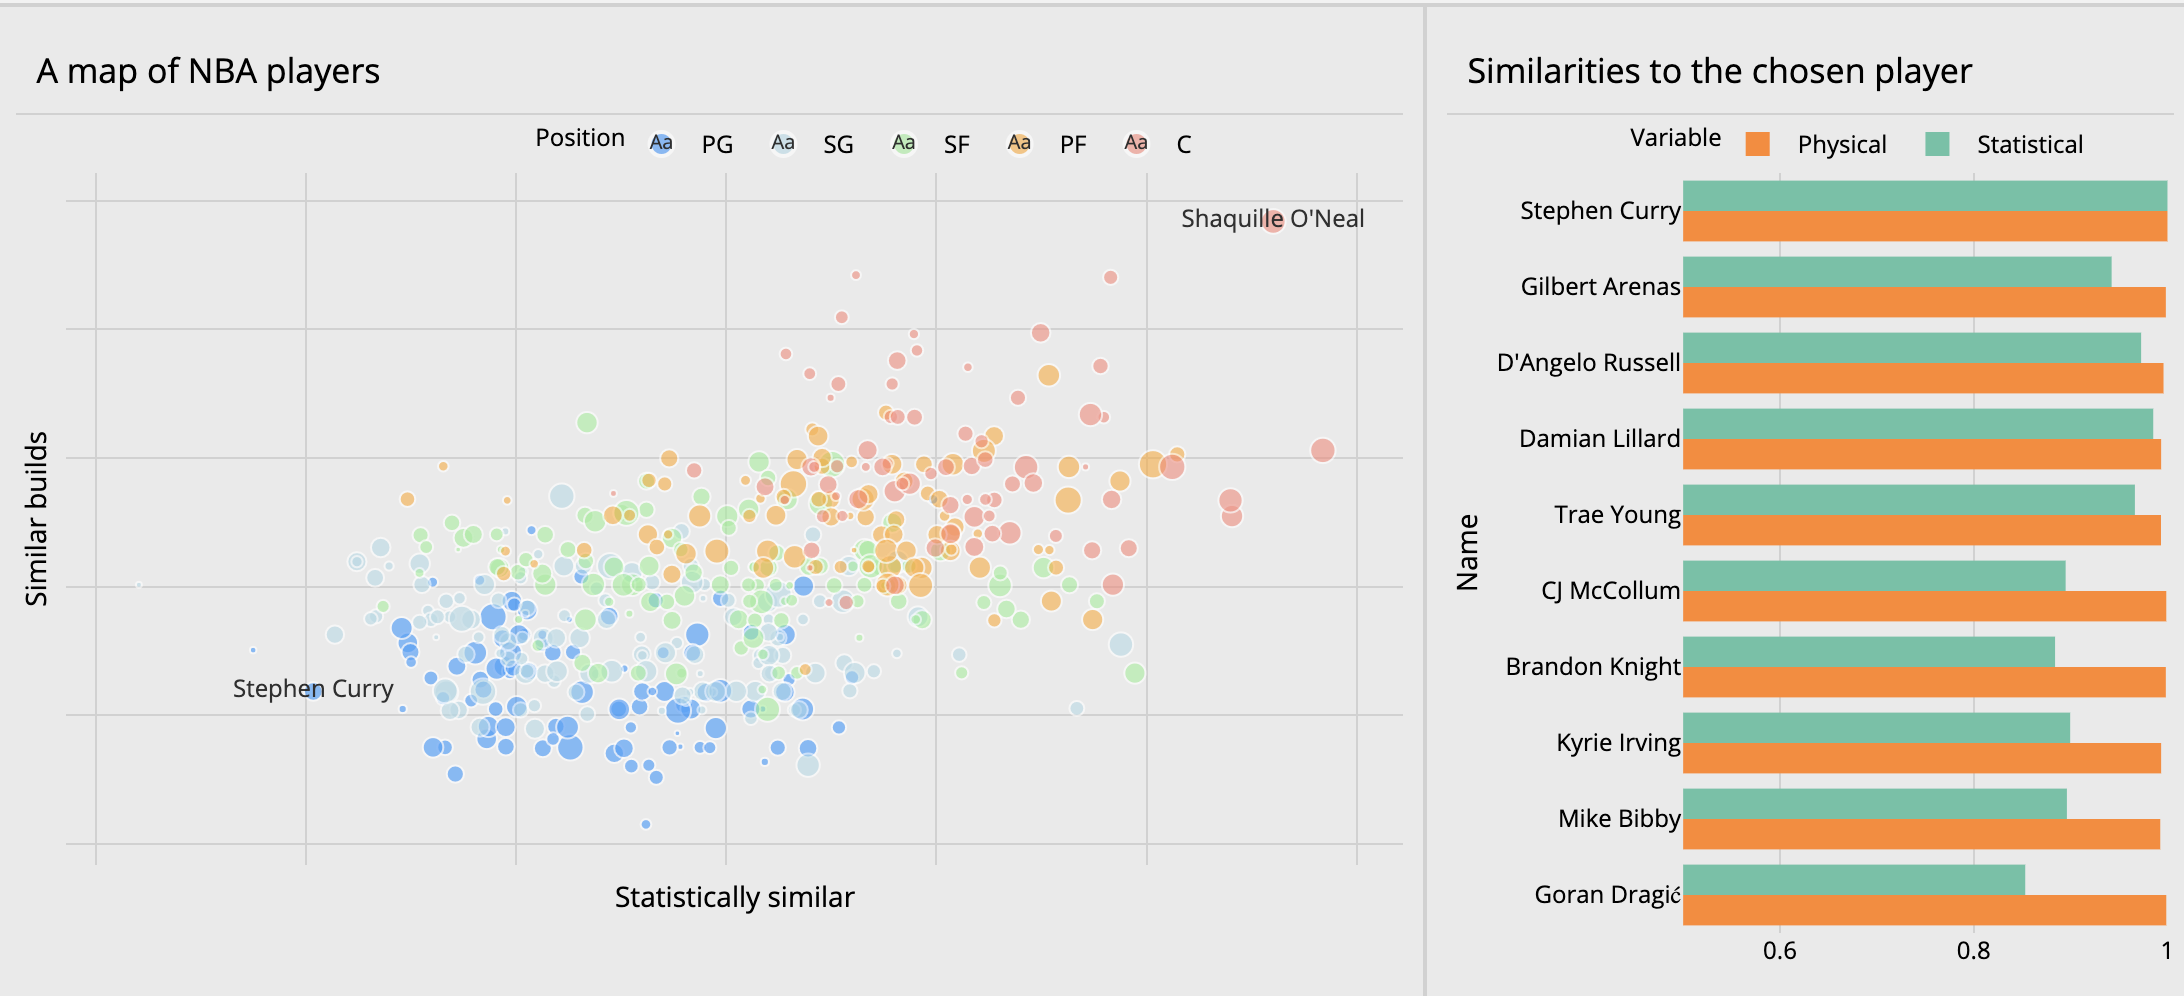
\includegraphics[width=.98\linewidth]{Steph_Comparisons.png}
    \caption{
        Steph Curry's Physical Comparison to other Players in the NBA 
    }
    \label{fig:second-page}
\end{figure}

Another work that is similar to my project is the website StatMuse created by Eli 
\textcite{statmuse}.
The user can use key words to look up stats for a team or players across all sports in America. It displays the stats the the user was looking for in a chart after the website finds the specific stats. Examples of specific stats can be a specific player vs a team in their career, most point in a game in a specific year and much more. The website also has fantasy sport projections that users can ask the website. It will display a projection number in a chart for the player they want to know about. Compared to what I want to do, I would simplify this by not using keywords to look up stats and display graphs of the data that the user want to visualize. In Figure 3, when looking up stats in Statmuse, you have to use key words and the words used are "steph curry playoff win loss record". With this, it shows the playoff record of Steph Curry's whole basketball career and the overall stats for those playoff games for each year he has gone to the playoffs. The inspiration for the Statmuse website comes from analysts and people that watch/engage in sports because of how these people want to find specific stats of players and teams that can be meaningful. An example would be finding out if a player does good in elimination games and can be evaluated based on those stats which are negative, neutral, or positive. 

\begin{figure}
    \centering
    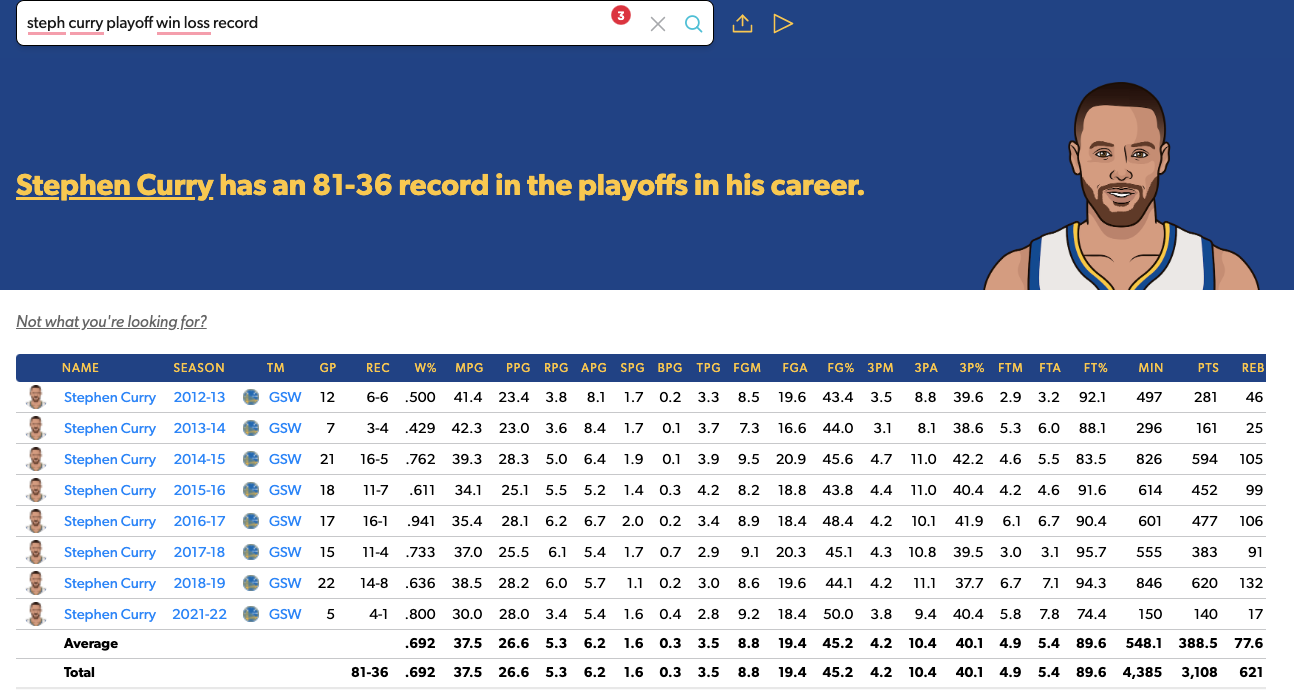
\includegraphics[width=.98\linewidth]{StatsMuse_Curry.png}
    \caption{
        Steph Curry's Playoff W/L Record with Stats
    }
    \label{fig:second-page-2}
\end{figure}

\section{Methods}

What I plan on doing for collecting the NBA stats for my project would be to query them from sports stats database like SportsReference. I would have to make an algorithm to pull these stats from the website based on what player the user chooses like "Stephen Curry" or "Lebron James" and what stats they specifically choose to evaluate the players and make comparisons.

For how the statistical data is going to be calculated and shown on a graph/chart, I need to create an algorithm using python to create and display data on a graph and show the stats used on a chart below. A mathematical model would need to be used for the data/stats and how to calculate them to make them used as a value for the player's value.

Datasets of surveys of people who might want to use my app for fantasy to look for the value of players will be useful for my project methods because of what they would want the user interface to have to make it easy to evaluate the data. 


\section{Evaluation}

For this summer to evaluate my project, I would do mock fantasy drafts and simulate the fantasy seasons based on the 2021-22 season to see results using my project to pick players. My project would be used to find a player with the specific stats that the user wants to take advantage of when other similar players are taken off the board like a superstar. The fantasy season would be simulated to see what place the user got in fantasy and to see if the players that were recommended had a positive impact on their team. I would calculate the place of the user's team and what percentage of points the players chosen based on my project created for the user's team. 

\printbibliography 

\end{document}